\documentclass[a4paper, 10pt]{article}
\usepackage[utf8]{inputenc}
\usepackage{verbatim}
\usepackage{listings}
\usepackage{graphicx}
\usepackage{a4wide}
\usepackage{color}
\usepackage{amsmath}
\usepackage{amssymb}
\usepackage[dvips]{epsfig}
\usepackage[toc,page]{appendix}
\usepackage[T1]{fontenc}
\usepackage{cite} % [2,3,4] --> [2--4]
\usepackage{shadow}
\usepackage{hyperref}
\usepackage{titling}

\setlength{\droptitle}{-10em}   % This is your set screw

\setcounter{tocdepth}{2}

\lstset{language=c++}
\lstset{alsolanguage=[90]Fortran}
\lstset{basicstyle=\small}
\lstset{backgroundcolor=\color{white}}
\lstset{frame=single}
\lstset{stringstyle=\ttfamily}
\lstset{keywordstyle=\color{red}\bfseries}
\lstset{commentstyle=\itshape\color{blue}}
\lstset{showspaces=false}
\lstset{showstringspaces=false}
\lstset{showtabs=false}
\lstset{breaklines}
\title{FYS3150 - Project 2}
\author{Daniel Heinesen, Halvard Sutterud, Gunnar Lange}
\begin{document}
\maketitle
\begin{abstract}We investigate a numerical solution to Schroedinger's equation for two electrons confined in a three-dimensional harmonic oscillator well. We present a solution to the case where we disregard the interaction between the electrons, and a solution where we include a repulsive (Coloumb) interaction between the electrons. 
\end{abstract}

\tableofcontents

\section{Introduction}
The study of electrons confined in a potential trap is a highly active research field today \textbf{INSERT SOME REFERENCES HERE}, due to its potential applicability in solid-state physics. Some proposed applications for these systems include semi-conductors and quantum gates for future quantum computers, as well as nano-medical applications.\\
\linebreak
We investigate Schroedinger's equation for two non-interacting electrons confined in a three-dimensional potential well, and reformulate it as an Eigenvalue problem. We then solve this problem by use of Jacobi's method for finding eigenvalues and eigenvectors. Once we have developed this general method, it is straightforward to implement the potential for the interacting electrons.

\section{Theoretical model}\label{Theoretical_section}
\subsection{Introducing the relevant Schroedinger equation}
A three-dimensional potential well is described by the harmonic oscillator potential:
\begin{equation}
V(r)=\frac{1}{2}kr^2
\end{equation} 
Here $r$ is the distance from the origin, and $k$ is a constant describing the steepness of the well. Note how this potential is radially symmetric. This means that we can ignore the angular parts of the Schroedinger's equation, leaving us with the radial equation:
\begin{equation}
-\frac{\hbar^2}{2m}\left(\frac{1}{r^2}\frac{d}{dr}r^2 \frac{d}{dr}-\frac{l(l+1)}{r^2}\right)R(r)+V(r)R(r)=ER(r)
\end{equation}
Here $E$ is the energy of the harmonic oscillator, and $l$ are orbital momentum numbers\footnote{Our background in quantum mechanics being nonexistent, we assume this sentence to be meaningful.}. Substituting $R(r)=\frac{u(r)}{r}$ as done \textbf{INSERT REFERENCE HERE}, we obtain:
\begin{equation}\label{eq:Radial_Schroedinger}
-\frac{\hbar^2}{2m}\frac{d^2}{dr^2}u(r)+\left(V(r)+\frac{l(l+1)}{r^2}\frac{\hbar^2}{2m}\right)u(r)=Eu(r)
\end{equation}
From this transformation, it also follows that the boundary conditions are necessarily $u(0)=u(\infty)=0$.
\subsection{Reformulating the equation as an Eigenvalue problem}
After some rescaling of equation \ref{eq:Radial_Schroedinger} described \textbf{HERE}, we can reformulate equation \ref{eq:Radial_Schroedinger} as:
\begin{equation}
-\frac{d^2}{d\rho^2}u(\rho)+V(\rho)u(\rho)=\lambda u(\rho)
\end{equation}
Where $\rho$ is a dimensionless quantity describing a characteristic length and $\lambda$ are the (sought-after) eigenvalues of the system. $V$ is the chosen potential. To reformulate this as an Eigenvalue problem, we discretize the second derivative. This implies that we write the continuous function $u(\rho)$ as a function at discrete points, $u(\rho_i)=u_i$, with $i=0,1,...,N$. We can then expand the second derivative in terms of Taylor polynomials to get an iterative scheme for solving the differential equation. The detailed procedure can be found \textbf{HERE}, with the final result:
\begin{equation}
d_iu_i+e_{i-1}u_{i-1}+e_{i+1}u_{i+1}=\lambda u_i
\end{equation}
Where  $d_i=2/h^2+V_i$ and $e_i=-1/h^2$, with $h$ being the step length (distance between $\rho_i$ and $\rho_{i+1}$). Note how every $e$ is the same, i.e. we can define $e_i=e$. This can now be reformulated as an eigenvalue problem with a tridiagonal matrix, $\mathbf{A}$ that is:
\begin{equation}\label{eq:Eigenvalue_problem}
\mathbf{A}\mathbf{u}=\lambda \mathbf{u}
\end{equation}
The matrix $\mathbf{A}$ is found by inserting the $u$ and $e$ from above, giving:
$$\mathbf{A}=\begin{bmatrix}
d_0 & e & 0 & 0 & \dots & 0 & 0\\
e & d_1 & e & 0 & \dots & 0 & 0\\
0 & e & d_2 & e & 0 \dots & 0\\
\dots & \dots & \dots & \dots & \dots& \dots & \dots \\
0 & \dots & \dots &\dots & e & d_{N-1} & e\\
0 & \dots & \dots & \dots & \dots & e & d_N\\
\end{bmatrix}$$
Note, however, that $u_0$ and $u_N$ are known, and thus we can remove those rows and columns from the matrix.
\subsection{Jacobi's algorithm for solving an eigenvalue problem}
Equation \ref{eq:Eigenvalue_problem} can be solved via a general algorithm known as Jacobi's method. Details of this method can be found \textbf{HERE}, but the general idea is rather straightforward. 
\subsection{Investigating the properties of orthogonal transfomrations}
We will here briefly investigate some properties of orthogonal transforms, to arrive at possible unit tests to implement in our programs. 
We will show that this transformation preserves the dot product and orthogonality. Thus let $\mathbf{v}_i$ and $\mathbf{v}_j$ be two arbitrary vectors. Consider an orthogonal transformation matrix, $\mathbf{U}$, that is $\mathbf{U}^T=\mathbf{U}^{-1}$. Define $\mathbf{w}_i=\mathbf{U}\mathbf{v}_i$ and $\mathbf{w}_j=\mathbf{U}\mathbf{v}_j$. Consider:
$$\mathbf{w}_i \cdot \mathbf{w}_j=\left(\mathbf{U}\mathbf{v}_i\right)^T\left(\mathbf{U}\mathbf{v}_j\right)$$
Where the last equality follows from the definition of the inner product. Using the properties of the transpose, the first parenthesis can be expanded as:
$$\left(\mathbf{U}\mathbf{v}_i\right)^T = \mathbf{v}_i^T\mathbf{U}^T$$
Multiplying this out gives:
$$\mathbf{w}_i\cdot \mathbf{w}_j=\mathbf{v}_i^T\mathbf{U}^T\mathbf{U}\mathbf{v}_j=
\mathbf{v}_i^T\mathbf{I}\mathbf{v}_j=\mathbf{v}_i\cdot \mathbf{v}_j$$
This shows immediately that the orthogonal transformation preserves the dot product. It also shows, however,that it prerves orthogonality. To see this, assume therefore that we have a basis of orthonormal vectors, $\mathcal{B}=\{\mathbf{v}_i\}$, i.e. that $\mathbf{v}_i\cdot \mathbf{v}_j=\delta_{ij}$. Inserting this into the last expression gives:
$$\mathbf{w}_i\cdot \mathbf{w}_j=\delta_{ij}$$
Which shows that orthogonal transformations also preserve orthogonality between vectors.



\section{Results}

After solving the the Schrödingers equation for both the 2 interacting electrons and 2 non-interacting electrons, for four different frequencies for the harmonic oscillator $\omega_r$, we get these graphs(\textbf{FIG1}).\\

\begin{figure}
\begin{center}
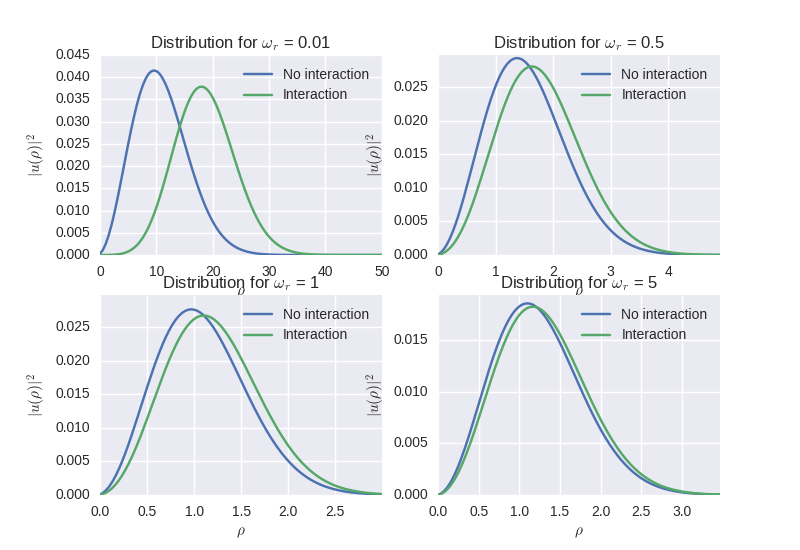
\includegraphics[width=70mm]{distribution_subplot.png}
\caption{Plots showning the probability distribution for the relative position of the two electrons. Omega corresponds to the frequency of the harmonic oscillator potential, which can be seen as the width of the potential well.}\label{fig:finfigur}
\end{center}
\end{figure}

As can be seen, the larger $\omega_r$ is, the closer $|u(\rho)|^{2}$ for the interacting and non-interacting electrons are; $|u(\rho)|^{2}$ being the probibility distribution for the relative position of the two electrons. We can interpet these results by looking at the different i potential energy in the two cases:

\subsection{Non-interacting}

In the non-interaction case the only potenial energy is the harmonic oscillator potential, given dimensionless as: (\textbf{IKKE SIKKERT VI TRENGER Å GJENGI FORMELENE HER, OM DE ER DEFINERT TIDLIGERE I ARTIKKELEN})

$$
V(\rho) = \omega\rho^{2} 
$$

$\omega$ will determine the width of this potential well, and therefor determine the probability of the relative distance for the electron: the greater $\omega$ is, the smaller the narrower the potenial well is and the closer the electrons are probable to be eachother. This is also what we see in the results.

\subsection{Interacting}

It the interacting case, we have two potenials competing, the harmonic oscillator potential (HO) and the coloumb potential, given by

$$
V(\rho) = \underbrace{\omega\rho^{2} }_{HO} + \underbrace{1/\rho}_{Coloumb}
$$

As mentioned above, for larger $\omega$ the closer the interacting solution is to the non-interacting solution. If we look at the two parts of the potential, we can see that for small a $\rho$, the Coloumbs potential is dominant, and for larger $\rho$, the HO is dominant. We can find that the $\rho$ where domain where the coloumb potential is dominant is

$$
\rho < \omega_r^{-\frac{1}{3}}
$$ 

This means that the larger $\omega_r$ is, the larger the domain where the coloumb potential is dominant is, and thus we expect a greater probablity for a greater relative distance between the two electrons. This is exactly what can be seen from the results. For the larger $\omega$'s the HO well is quite small, and is therefor wholy dominant, causing the solutions for both potenitals to be similar. For smaller $\omega$'s the HO wells are large and the electrons have the posibility to have a large relative distance from eachother.


\section{Methods}
The program used to solve these equations mainly consisted of two classes. We used one class for solving the Schrödinger equation for a given potential. This class calculates the matrix elements described above and returns the matrix. The second class uses Jacobi's method to solve the eigenvalue problem. Most of the code for Jacobi's method was heavly inspired by code found \textbf{HERE}\\

For different values for $\omega_r$ the width of the probability distribution varies, and becomes larger for smaller $\omega_r$. To get the best resolution without having to decrease the step length, a $\rho _{max}$ had to be choose for each $\omega_r$, mostly by trial and error.\\

We chose to look at four different values for $\omega_r$ between $0.01$ and $5$. We only looked at the lowest state energy eigenfunction, and the difference between the interacting and non-interaction cases. The parameter used:\\

\begin{tabular}{|l||c|c|c|c|}
\hline
$\omega_r$ & 0.01 & 0.5 & 1 & 5 \\
\hline
$\rho_{max}$ & 50 & 10 & 10 & 5 \\
\hline
\end{tabular}\\

With a mesh grid dimensionality of 200. \\

To ensure that the code behaved as we wanted, we implemented two unit test. The first unit test ensures the conservation of inner product of vectors given by $\mathbf{w}_i = \mathbf{A}\mathbf{v}_i$ after each similarity transformation done to $\mathbf{A}$. 

\lstinputlisting{psudo_code1.cpp}



The second unit test ensures that the method used to find the largest non-diagonal element in the matrix gives the correct element.

\lstinputlisting{psudo_code2.cpp}


\end{document}
